\documentclass[a4paper]{report}

\usepackage{graphicx}
\usepackage{amsmath, amsthm}

% To get slightly smaller margins
\usepackage{fullpage}

% To get paragraphs right
\usepackage[parfill]{parskip}

% Correct input encoding
\usepackage[utf8x]{inputenc}

% For URL:s
\usepackage{url}

% For subfigures
\usepackage{subfig}

\begin{document}

\title{FlaXx: A Monte-Carlo (Stochastic) Ray Tracer}
\author{Nathalie Ek \and Albert Cervin}

\maketitle

\begin{abstract}
The problem of global illumination has existed a long time and many
different solutions have been proposed. The first usable solution that
produced good results was proposed by Turner Whitted \cite{whitted} in
1980. Other people improved his work and the Monte Carlo method was
incorporated into ray tracing, producing an algorithm known as
stochastic ray tracing. This article describes an implementation of
such a ray tracer. It incorporates the Monte Carlo scheme both for
sampling shadow rays and directions for indirect rays. The result is a
computationally heavy algorithm that will for a high number of samples
per pixel converge towards an accurate solution. Different experiments
were carried out varying parameters for the rendering. The conclusion
is that the number of viewing rays have the biggest impact on the
final result. To achieve an even more realistic result, photon mapping
should be implemented.
\end{abstract}

\tableofcontents

\listoffigures

\chapter{Introduction}

\section{Global Illumination}

The problem of global illumination has existed just as long as images
have been produced with computers. The problem consists of solving the
rendering equation. The hemispherical formulation of the rendering equation is

\begin{equation}
  L(x \to \Theta) = L_e(x \to \Theta) + \int_{\Omega_x}f_r(x,\Psi \to \Theta)L(x \gets \Psi)\cos{N_x,\Psi}d\omega_\Psi
  \label{eq:renderingeq}
\end{equation}

where \(L(x \to \Theta)\) is the radiance going from the point \(x\)
in direction \(\Theta\), \(L_e(x \to \Theta) \) is the self-emitted
radiance from the point \(x\) in direction \(\Theta\), \(f_r(x,\Psi
\to \Theta)\) is the Bidirectional Reflectance Distribution Function
(BRDF) which tells how much of the incoming light from direction
\(\Psi\) to the point \(x\) is leaving in direction \(\Theta\). The
BRDF is material-dependent and will look different for different materials.

\subsection{Whitted Ray tracing}

The first usable solution to this problem was proposed by Turner
Whitted \cite{whitted} in 1980. Whitted proposed a ray-tracing scheme
where only perfect specular reflection and refraction is
considered. This means that in each intersection point, one reflected
and one refracted ray are spawned. This results in a recursive
solution to the rendering equation (\ref{eq:renderingeq}). To take
diffuse interactions into consideration, a local
lighting model is used where rays are cast towards the light source
from the ray intersection point with an object. This solves the
problem with shadows and diffuse objects. However, this method stops
the recursion as soon as a diffuse surface is hit and thus does not
take diffuse interreflections into consideration.

\subsection{Radiosity}

Another method that takes diffuse interreflections into consideration
is the radiosity method, proposed by Goral et al. \cite{goral}. The
radiosity method divides the scene into patches and a set of equations
is set up, based on the conservation of light energy. The light transport
between these patches are then calculated. Every patch in the
environment gets reflected light from all other patches in the
scene. A patch can also emit light if it is a light source. This is
represented by the radiosity formula.

\begin{equation}
  B_i = E_i + R_i\sum^n_{j=1}B_jF_{ij}
  \label{eq:radiosity}
\end{equation}

In this equation (\ref{eq:radiosity}), \(B_i\) is the radiosity for
patch \(i\), \(E_i\) is the energy emitted from the same patch,
\(R_i\) is the reflectivity of the patch and the sum is a sum over all
the other patches radiosity \(B_j\), weighted by the form factor
between patch \(i\) and \(j\), \(F_{ij}\). Equation \ref{eq:radiosity}
exists for every patch present in the scene and therefore the solution
to this equation becomes the solution of a set of \(n\) simultaneous equations.

The form factors, as stated above, take the geometric relation between
two patches into consideration. It can be noted that \(F_{ii} = 0 \)
for a plane and convex surface. In words, the calculation of the form
factors can be expressed as

\begin{equation}
  F_{ij} = \frac{\text{Radiative energy leaving surface } A_i \text{ that
    strikes } A_j \text{ directly}}{\text{Radiative energy leaving
    surface } A_i \text{in all directions in the hemispherical space
    surrounding } A_i}
\end{equation}.

\subsection{Monte Carlo ray tracing}

This method is also called stochastic ray tracing. Essentially it is
an application of Monte Carlo integration methods in 3D computer
graphics. Instead of just considering one reflected and one refracted
ray in intersections as is the case with Whitted ray tracing, many
rays are considered (sampled). The same method for shadows and direct
illumination is used where shadow rays are shot towards the
light source to determine visibility (shadows) and illumination. The
indirect illumination scheme is quite different from the Whitted
scheme, though. When a ray intersects a surface in the scene, the
material properties are considered and according to that multiple rays
are cast. The most important directions for the final image have a
higher probability of being sampled. This is in Monte Carlo methods
known as importance sampling, which simply means that more important
directions are sampled more frequently in a ray tracer. This yields a
lower variance meaning that the method will converge to an accurate
solution of the equation faster.

Monte Carlo integration techniques rely on the relation saying that the expectation value
of an estimator is exactly the value of the integral.

If we have an integral \(I\), the estimator \(\langle I \rangle\) is

\begin{equation}
  \langle I \rangle = \frac{1}{N}\sum^N_{i=1}\frac{f(x_i)}{p(x_i)}.
  \label{eq:estimator}
\end{equation}

It can be shown that 

\begin{equation}
  E[\langle I \rangle] = I
\end{equation}

where \(I\) is the integral to be estimated.

This shows that the more samples used in the estimator, the more
accurate is the estimation of I.

Since ray tracing is a recursive procedure, the tracing has to be
stopped at some point. If this is done by limiting the recursive depth
to a constant number, the image will be biased and there will be
visible effects in the final image. Instead a stopping condition
called Russian roulette is used. This means that in each ray
intersection there is a certain probability for the evaluation to
stop. This way, the recursive depth can depend on for instance the
local hemispherical reflectance of the surface hit by a ray. Russian
roulette will produce an unbiased image.

To get rid of aliasing effect and to further lower the variance, many
rays are shot into the scene per pixel. In this way the need for
spawning many rays at each intersection point diminishes and therefore
few rays are spawned at the intersection point and instead more
viewing rays are used. With stochastic (Monte Carlo) raytracing it is
hard to model caustic effects though but this can be done with another
global illumination method called photon mapping.

\subsection{Photon mapping}

Photon mapping was proposed as a global illumination algorithm by
Henrik Wann Jensen \cite{jensen} in 1996. Rays from the light source
and from the camera are traced independently and then combined in a
second step to produce a radiance estimate. This makes it possible to
simulate reflection and refraction in a better way, taking caustics
into consideration. Photon mapping is a ``biased'' algorithm meaning
that more passes of the algorithm will not give a more accurate
solution. Using more photons will however give a more correct solution.

The first pass in the algorithm is creating the photon maps. Photons
are sent out from the light sources and when the photon intersects an
object in the scene, the intersection point and the incoming direction
is stored in a cache called the photon map. After this, Russian
roulette (see above) is used to evaluate the next action for the
photon: absorption, transmission or reflection. The photon map is
typically stored in a kd-tree for fast nearest neighbor searching. The
map is then stored for later use.

The second pass is a ray tracing pass where a ray is shot from the
camera and then an intersection point is found. Direct illumination in
this point is evaluated with the same scheme as in the above ray
tracing algorithms. For indirect illumination however, the photon map
is used. Specular reflection is handled well by standard ray tracers
and is therefore done by the ray tracing algorithm. For soft indirect
illumination, the global photon map is used. For caustics, the other
photon map, called the caustic photon map is used.

In order to calculate surface radiance at an intersection point, one
of the cached photon maps is used. The steps are:

\begin{enumerate}
\item{Gather the N nearest photons using the nearest neighbor search function on the photon map.}
\item{Let S be the sphere that contains these N photons.}
\item {For each photon, divide the amount of flux (real photons) that
    the photon represents by the area of S and multiply by the BRDF applied to that photon.}
\item{The sum of those results for each photon represents total
    surface radiance returned by the surface intersection in the
    direction of the ray that struck it.}
\end{enumerate}

\section{Introduction}
This first section is an introduction to the global illumination problem and different
solutions proposed. In the next chapter Monte Carlo ray tracing will be
discussed more in detail, and details of our implementation will be
presented. In chapter \ref{ch:results} results from the implementation
is presented and discussed. Discussion and outlook is presented in chapter \ref{ch:discussion}. 

\chapter{Background}

A Monte Carlo ray tracer has been implemented in C++ and here the
implementation details will be presented. The algorithm will be
described in the order it runs. That is, first the camera and the view
plane is described, then ray-surface intersections and after that the
calculation of direct and indirect illumination in a given
intersection point.

\section{Setting up the render}

The first thing is to create a render object which will hold and
gather all information regarding the render. This is created with
options from the command line provided by a user. The number of
viewing rays, number of shadow rays, number of indirect rays, image
dimensions etc. can be specified. The render object also creates an
image plane object which is responsible for providing world
coordinates for a pixel and for dividing the image into a number of
tiles to be rendered. This is illustrated in figure
\ref{fig:camera}.

\begin{figure}
  \centering
  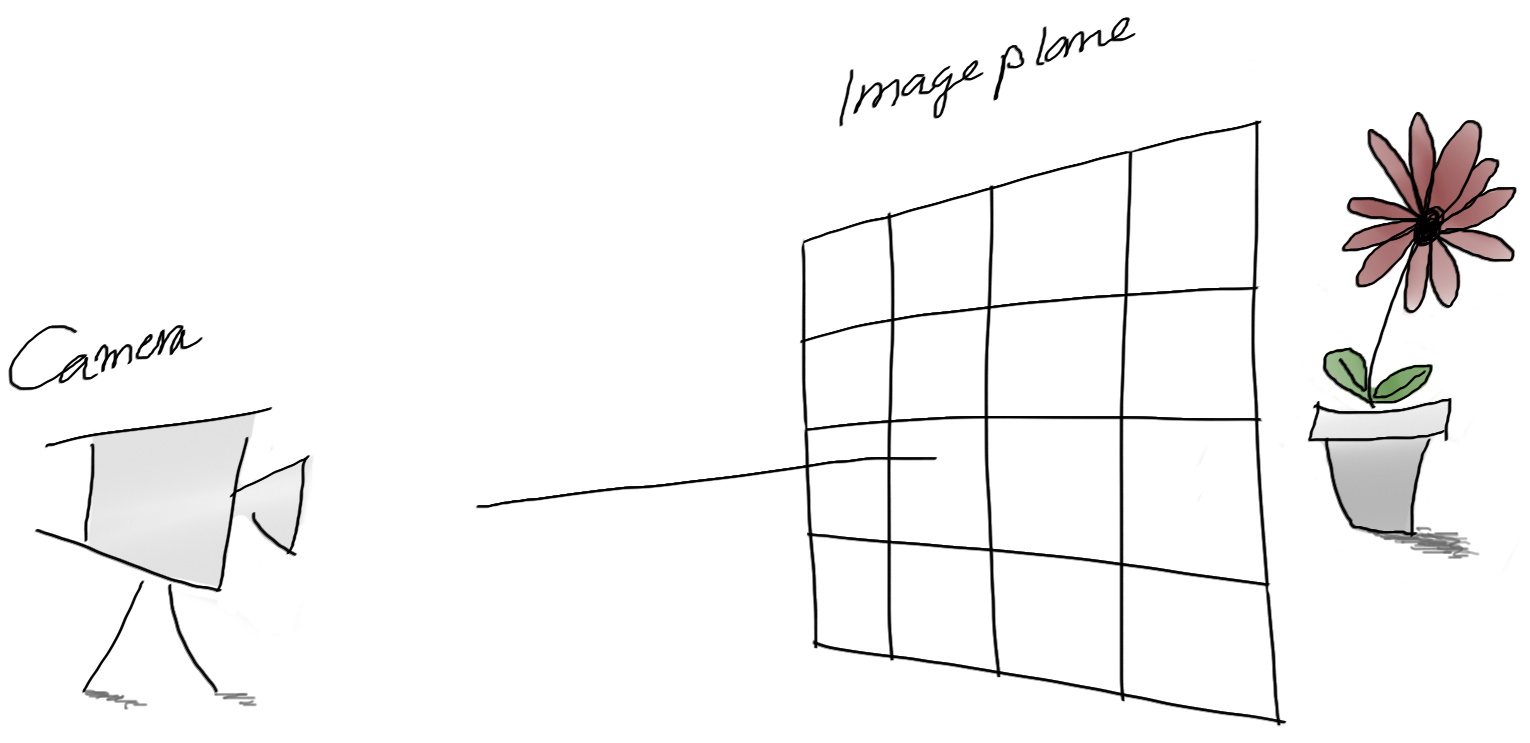
\includegraphics[width=10cm]{figures/2}
  \caption{Camera and image plane set-up.}
  \label{fig:camera}
\end{figure}

The pixels in the image are divided into ten tiles in \(x\)-direction and
a corresponding number to have the tiles quadratic, in
\(y\)-direction. The tiles closest to the middle of the image are
selected for rendering first, since the middle of the image are in
most cases the most interesting. This way there is no need to sit and
wait for the render to reach the middle of the image. The middle in
this case means the center of the image in \(x\)-direction.

\section{Camera and view plane}
\label{sec:cam}

The camera is placed by default in the origin \((0, 0, 0)\) and the
viewing direction is by default in positive \(z\)-direction. That
means that positive \(Z\) is into the screen. The view plane is
defined to have a width that can be varied by varying the field of
view for the camera. The camera also has a depth of field setting that
can be varied to achieve different depth field effects \footnote{Not
  currently implemented}.

Multiple rays can be shot through each pixel and stratified sampling
is used to avoid clamping of samples in the pixel. The pixel is
subdivided into the nearest even square number of the number of
viewing rays requested. For example, if 1000 viewing rays are
requested, the pixel is subdivided into \(\lceil \sqrt{1000}
\rceil^2 = 1024 \) subpixels. A ray is then shot through a jittered
center point of the sub-pixel. This gives a result as in figure \ref{fig:jittered}.

\begin{figure}
  \centering
  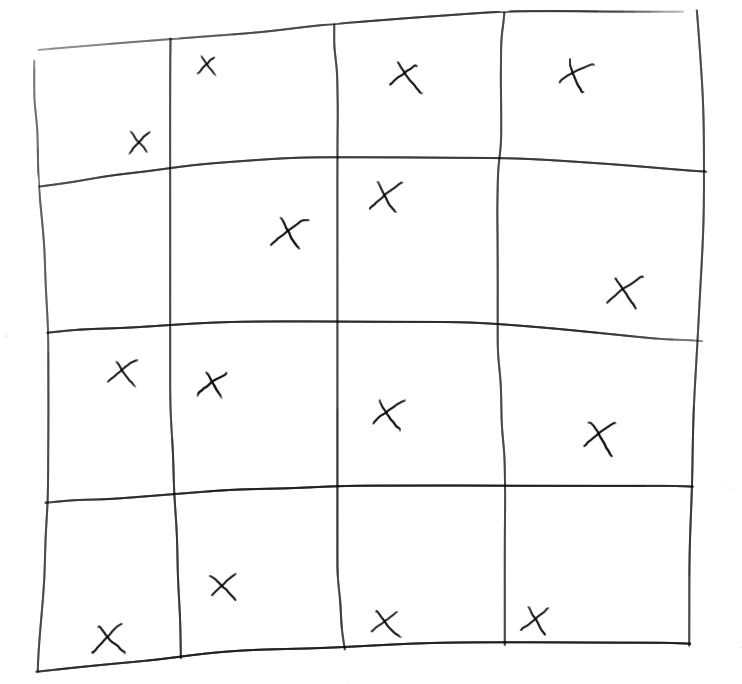
\includegraphics[width=10cm]{figures/1}
  \caption{Stratified (jittered) sampling.}
  \label{fig:jittered}
\end{figure}

\section{Intersection tests}

The scenes in this implementation consists of spheres, planes and
polygonal objects \footnote{Planned}. Intersections between rays and
these object has to be carried out.

\subsection{Ray-triangle intersection}

To check if a ray intersects a triangle has to be done for both planes
(which consists of two triangles) and for polygonal objects. These
tests are done with barycentric coordinates \cite{pointTest:10}. First, a point on the ray
is projected onto the same plane as the triangle lies in:

\begin{equation}
  P = R_o - R_d\frac{(R_o-v_1) \cdot N}{R_d \cdot N}
  \label{eq:planeproj}
\end{equation}

where \(P\) is the resulting point, \(R_o\) is the origin of the ray
\(R\), \(R_d\) is the direction of the same ray, \(v_1\) is the first
vertex on the triangle and \(N\) is the normal of the triangle.

After this the sides of the triangle is parametrized into \(u\) and
\(v\). To do this, intermediate vectors \(i_1\), \(i_2\) and \(i_3\)
are created as follows:

\begin{align}
  i_1 &= v_2 - v_1 \nonumber \\
  i_2 &= v_3 - v_1 \nonumber \\
  i_3 &= P - v_1
  \label{eq:intermediate}
\end{align}

where \(v_i\) is vertex point \(i\) on the triangle and \(P\) is the point calculated
in equation \ref{eq:planeproj}. Now \(u\) and \(v\) can be calculated:

\begin{align}
  u &= \frac{(i_2 \cdot i_2)(i_1 \cdot i_3) - (i_1 \cdot i_2)(i_2
    \cdot i_3)}{(i_1 \cdot i_1)(i_2 \cdot i_2) - (i_1 \cdot i_2)(i_1
    \cdot i_2)} \nonumber \\
  v &= \frac{(i_1 \cdot i_1)(i_2 \cdot i_3) - (i_1 \cdot i_2)(i_1
    \cdot i_3)}{(i_1 \cdot i_1)(i_2 \cdot i_2) - (i_1 \cdot i_2)(i_1
    \cdot i_2)}.
  \label{eq:uandv}
\end{align}

After calculation \(u\) and \(v\) the only thing left is to check that
\(u,v \geq 0\) and that \(u+v \leq 1\). If that is the case, the ray
is intersecting the sphere. A situation where this holds is
illustrated in figure \ref{fig:pointintriangle}.

The camera setup is illustrated in figure
\ref{fig:camera}.

\begin{figure}
  \centering
  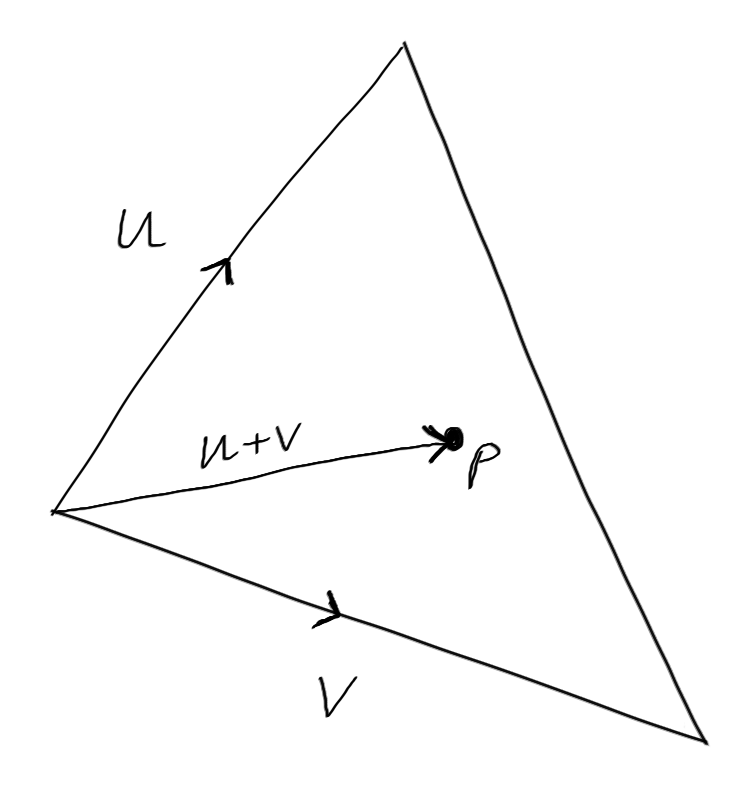
\includegraphics[width=7cm]{figures/3}
  \caption{A point P that is inside the triangle}
  \label{fig:pointintriangle}
\end{figure}

For planes, this test has to be done for both triangles in the plane
since the planes are essentially polygonal objects with two polygons.

\subsection{Ray-sphere intersection}

In this implementation spheres are implicit object (as opposed to
polygonal ones) and to calculate intersection with such a sphere the
distance \(D\) from the ray start \(R_o\) and the sphere center \(S_c\) is
calculated. A parameter \(b\) is also calculated 

\begin{equation}
 b = D R_d
 \label{eq:b}
\end{equation}

where \(R_d\) is the ray direction.

After this it can be checked that \(b \geq 0\) and that \(D \leq
radius^2\). If that is not true, the ray does not intersect the
sphere.

If the above is true though, further calculations has to be carried
out. An additional parameter \(c\) is calculated

\begin{equation}
  c = D - b²
\end{equation}

where \(D\) is the distance calculated above and \(b\) is the
parameter calculated in equation \ref{eq:b}.

Another check can now be performed to see that \(c \leq radius^2\). If
that is not true, there is no intersection.

Otherwise the intersection point is

\begin{equation}
  d = \sqrt{radius^2 - c}
  \label{eq:d}
\end{equation}

\begin{equation}
  P = \left \{ 
  \begin{array}{l l}
    R_o + R_d *(b-d) & \quad D \geq radius^2 \\
    R_o + R_d *(b+d) & \quad \text{otherwise} \\
  \end{array} \right.
\end{equation}

where \(P\) is the resulting intersection point, \(R_o\) and \(R_d\)
is the origin and direction of ray \(R\), respectively, \(b\) is the
parameter calculated in equation \ref{eq:b} and \(d\) is the parameter
calculated in equation \ref{eq:d}.

In the current implementation light sources are deliberately excluded
from the intersection tests. This was done because the ability to have
objects represent light sources was wanted. Future improvements are
needed to make this work in a good way though. This will be discussed more in
chapter \ref{ch:discussion}.

\section{BRDF and materials}

Materials are implemented as separate object and every material
inheriting from the base material has to have a BRDF function telling
what color the object shall have in a specific point given incoming
and outgoing direction. Currently a Lambert and a modified Blinn-Phong
BRDF are implemented. Some experimenting with a Cook-Torrance shader
was also done but was put on the to-do-list.

Each material also has a color and if refractive properties are set
for the material, the refractive index has to be set.

The diffuse \(k_d\) and specular \(k_s\) components of the material
has in this implementation to always sum up to at most 1, since a
material with \(k_d = 0\) and \(k_s = 1\) is considered to be a
perfectly specular material. 

\section{Direct illumination}

After an intersection point has been found the direct illumination
contribution to that point is calculated. This is done by casting
multiple shadow rays towards the light source. If more than one light
source exist in the scene, one of the light sources are picked
uniformly with a random number. 

After the light source has been picked, a point on its surface is
sampled (in the case it is an area light source). This is also done uniformly.

The Monte Carlo estimator for direct illumination then becomes

\begin{equation}
  \langle L_{direct}(x \to \Theta) \rangle = \frac{N_L}{N}\sum^N_{i=1}
  A_{L_k}L_e(y_i \to \vec{y_ix})f_r(x,\Theta \leftrightarrow
  \vec{xy_i})G(x,y_i)V(x,y_i)
  \label{eq:direst}
\end{equation}

where \(N_L\) is the number of light sources, \(N\) is the number of
shadow rays, \(A_{L_k}\) is the area
of the light source, \(L_e\) is the emittance of the light source,
\(f_r\) is the BRDF of the surface, \(G\) is the geometry term and \(V\) is the
visibility term.

\(V\) and \(G\) are then left to be calculated. \(V\) is a boolean
term telling if the light source point \(y_i\) is visible from the
object point \(x\). If the light source point is visible \(V = 1\)
otherwise it is \(0\).

The geometry term \(G\) takes the geometric relation between point
\(x\) on the object and point \(y_i\) on the light source. It is
expressed as

\begin{equation}
  G(x,y_i) = \frac{(N_x \cdot \Psi)({N_Y}_i \cdot -\Psi)}{{r^2_{xy}}_i}
  \label{eq:geometry}
\end{equation}

where \(N_x\) is the normal at point \(x\), \(\Psi\) is the vector
between point \(x\) and \(y_i\), \({N_y}_i\) is the normal at point
\({N_y}_i\) and \({r^2_{xy}}_i\) is the square of the distance between
point \(x\) and \(y_i\).

After calculation of visibility and geometry everything needed for
calculating the direct illumination at point \(x\) is known. The
direct illumination is then added to the total estimated radiance.

This scheme can be summarized by the illustration in \ref{fig:direct}.

\begin{figure}
  \centering
  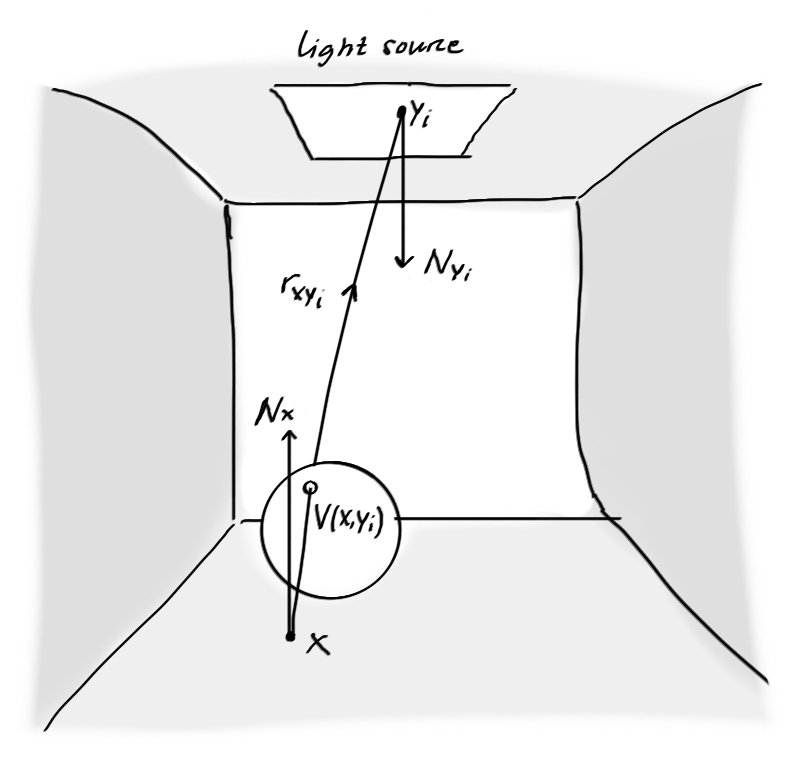
\includegraphics[width=10cm]{figures/4}
  \caption{Direct illumination algorithm.}
  \label{fig:direct}
\end{figure}

In figure \ref{fig:direct} the evaluation of \(V(x,y_i)\) can be seen
and \(y_i\) is a sampled point on the light source. \(N_x\) and
\({N_y}_i\) is the normals in the two points.

The algorithm is then repeated for the number of shadow rays decided
by the user of the software.

\section{Indirect illumination}

The next step in estimating the radiance is to evaluate the indirect
illumination at the intersection point \(x\). This is done by
evaluating the hemispherical integral in the rendering equation
(\ref{eq:renderingeq}). A Monte Carlo scheme is applied to this
integral since it is clear that no exact solution to this integral can
be achieved. The sampling schemes used are obtained from Dutré \cite{globalcomp}. 

The estimator for indirect illumination is

\begin{equation}
  \langle L_{indirect}(x \to \Theta) \rangle = \frac{1}{N}\sum^N_{i=1}
  \frac{L_r(r(x,\Psi_i) \to -\Psi_i)f_r(x,\Theta \leftrightarrow
    \Psi_i)(\Psi_i \cdot N_x)}{p(\Psi_i)}
  \label{eq:indirest}
\end{equation}

where \(N\) is the number of indirect rays, \(L_r\) is the reflected
radiance, \(f_r\) is the BRDF of the surface, \(\Psi_i\) is the
sampled hemisphere direction, \(N_x\) is the surface normal in the
point \(x\) and \(p(\psi_i)\) is the PDF \footnote{Probability Density
Function} used.

A recursive nature can be seen in the equation (\ref{eq:renderingeq})
and therefore a recursive algorithm suits well to solve the
equation. Russian roulette is used to determine the event at each
intersection point. The specular (\(k_s\)) and diffuse (\(k_d\)) components are summed up
to represent the local hemispherical reflectance. A uniform random
number is then generated and if the number is smaller than (\(k_d\)), a
diffuse reflection takes place. If the random number is larger than
 (\(k_d\)) but smaller than (\(k_s+k_d\)) a specular reflection or
 refraction takes place, depending on the reflective and refractive
 parts of the material. If the generated random number does not
 fulfill any of these two criteria, the ray is considered to be
 absorbed and the recursion is stopped. This imposes the condition
 that \(k_s+k_d \leq 1\). 

Directions on the hemisphere are sampled. In this
implementation importance sampling is done according to the following sections.

\subsection{Diffuse reflections}
For diffuse surfaces a cosine lobe around the normal in the point
\(x\) is used to spawn rays. The PDF for such a distribution of rays
is 

\begin{equation}
  p(\Theta) = \frac{n+1}{2\pi}\cos^n{\theta}
  \label{eq:cosnormal}
\end{equation}

where \(\theta\) is the incoming angle and \(n\) is a number between 0
and 1 to control the width of the cosine lobe. \(n=0\) gives a uniform
distribution around the whole hemisphere.

To sample directions according to equation \ref{eq:cosnormal} these
relations are used

\begin{align}
  \varphi &= 2 \pi r_1 \nonumber \\
  \theta &= \cos^{-1}(r_2^{\frac{1}{n+1}})
\end{align}

where \(r_1\) and \(r_2\) are two uniform random numbers and
\(varphi\) and \(\theta\) is the sampled hemispherical coordinates. The sampled
directions are then rotated to match the normal direction at \(x\).

\subsection{Specular reflections}

In the implementation, a specular component of 1 is considered to be a
perfect specular object and therefore a linear interpolation between a
sampled direction and the perfect reflection direction is made.

The interpolation can be described as

\begin{equation}
  D = k_sD_p + (1-k_s)D_s
\end{equation}

where \(D\) is the final direction, \(k_s\) is the specular
component of the material, \(D_p\) is the perfect specular reflection
direction and \(D_s\) is the sampled direction according to the
sampling scheme in equation \ref{eq:cossolid}.

The sampled direction is obtained by a cosine lobe around the perfect
reflection direction. The PDF for this sampling is

\begin{equation}
  p(\Theta) = \frac{\cos{\theta}}{\pi}
\end{equation}

where \(\theta\) is the incoming angle. To sample according to this
PDF equation \ref{eq:cossolid} can be used.

\begin{align}
  \varphi &= 2 \pi r_1 \nonumber \\
  \theta &= \cos^{-1}(\sqrt{r_2})
  \label{eq:cossolid}
\end{align}

where \(r_1\) and \(r_2\) are two uniform random numbers and
\(varphi\) and \(\theta\) is the sampled hemispherical coordinates. The sampled
directions are then rotated to match the perfect reflection direction
at \(x\).

\subsection{Specular refractions}

Russian roulette is used to determine the type of event at point \(x\)
so if the object is specular, the type of action (reflection or
refraction) is determined by comparing a uniform random number with
the transmission coefficient of the material. If the random number is
smaller, a refracted ray is constructed in exactly the same way as is
the case with specular reflections described in the section above.

However, the refracted direction is calculated according to Snells law
and before determining the event at point \(x\), a check to see if the
ray comes from inside or outside the object is made. If the ray comes
from the inside, a refracted ray out from the object is always
spawned.

When handling refractions, nothing can be assumed about the
transparent side of the BRDF so in this implementation a simple
constant is used as BTDF \footnote{Bidirectional Transmittance
  Distribution Function}.

\subsection{Recursive evaluation}

The radiance at point \(x\) is then calculated by shooting a ray in
the sampled direction and apply the same scheme there. The Russian
roulette scheme described above is used to determine the action in
each point. The number of sampled rays launched at each point is
pre-determined and this creates a recursive tree for indirect illumination.

\section{Setting the final color}

The indirect and direct illumination are summed together and is
then normalized linearly. SDL \cite{sdl} is used for
displaying a window and for saving the image to a png-file. After
normalization, values are set for the two SDL-surfaces (one for
display and one for saving to file). Then the
algorithm proceeds with the next viewing ray.

\chapter{Results and benchmarks}
\label{ch:results}

\section{Aliasing}

To get rid of aliasing effects in the image, jittered sampling is used
as described in section \ref{sec:cam}.

\begin{figure}
  \centering
  \subfloat[Without
  anti-aliasing]{\label{fig:alias}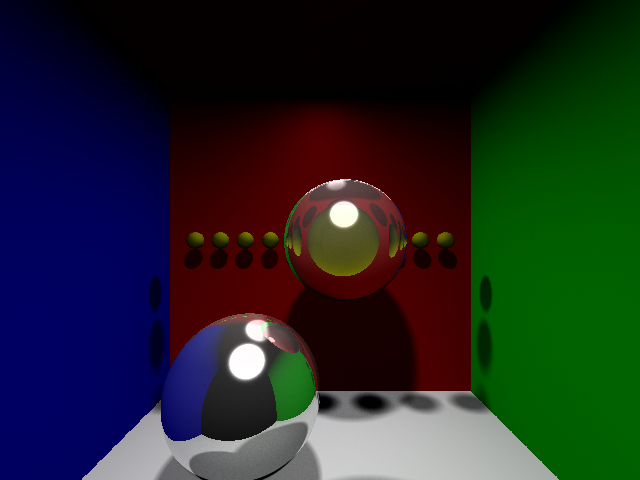
\includegraphics[width=8cm]{figures/500vr}}                
  \subfloat[With anti-aliasing]{\label{fig:aalias}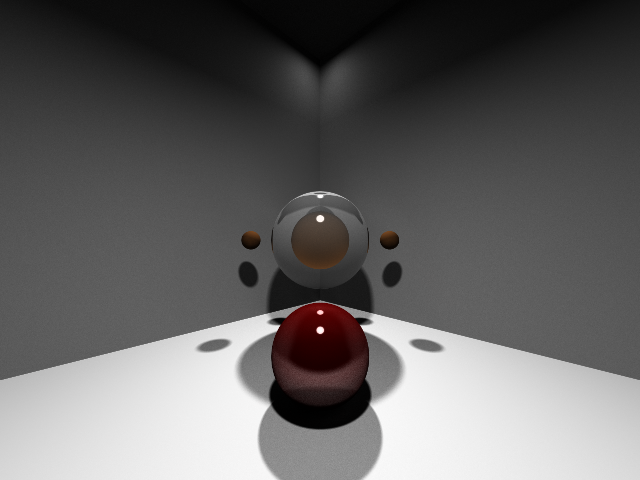
\includegraphics[width=8cm]{figures/aa}}
  \caption{Anti-aliasing vs Aliasing}
  \label{fig:aliasingcomp}
\end{figure}

The left image (\ref{fig:alias}) shows an image
without jittered sampling just shooting multiple rays through the
center of the pixel while the right image (\ref{fig:aalias}) shows an image where
jittered sampling is used. In figure (\ref{fig:alias}) the aliasing
effects can clearly be seen in the jagged edges in object boundaries
but can also clearly be seen where the walls meet the floor. This is
natural since the rays shot through the pixel always intersects with
the scene in the same way. 

When jittered sampling is used, the aliasing effects is
diminished. Both images in figure \ref{fig:aliasingcomp} have been
produced with 500 viewing rays. The problem with jittered sampling
though is that it uses \(N^2\) samples in the jitter. A possible
improvement to this could be to use N-rooks that only needs to use
\(N\) samples to achieve the same result. However this would result in
fewer indirect rays at each point and thus a less accurate solution to
the rendering equation.

\section{Obtaining an accurate solution}

The more rays used in the different stages of the algorithm, the more
accurate the solution will be. Since the algorithm itself is
stochastic, noise will be present. To lower this noise and produce a
nice image, multiple viewing rays has to be used. Averaging between
the radiance from these rays will give a kind of low-pass filtering of
the noise seen in images with fewer viewing rays. The more viewing
rays used, the better will the average be.

% Figur med olika många viewing rays

\section{Direct illumination}

The number of shadow rays greatly affect the shadow appearance in the
final image. More shadow rays produce a better result.

% Figur med olika många shadow rays

In these two images it can clearly be seen that more shadow rays gives
a smoother shadow, especially on the shadow edge. The reason for this
is that some sampled directions from the penumbra of the shadows will
be visible from the light source and some not. To produce a nice
average between those, more shadow rays has to be used. 

\section{Varying lights}

The color effects in the final image can be made clearer by changing
the color of one of the light sources in the scene.

% CHANGE THIS FIGURE
\begin{figure}
  \centering
  \subfloat[With white lights]{\label{fig:white}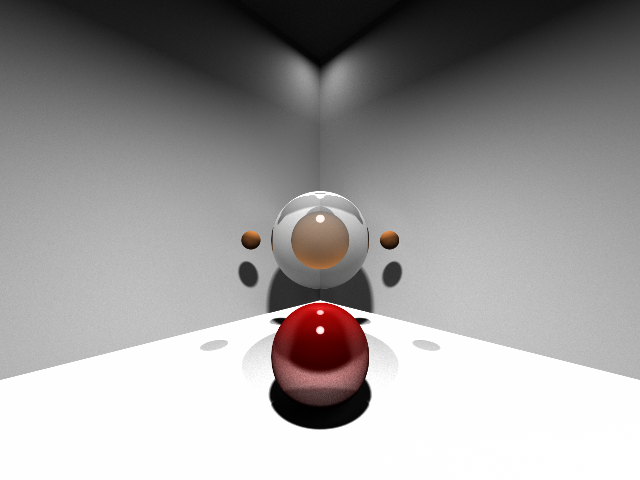
\includegraphics[width=8cm]{figures/white_light}}                
  \subfloat[With one pink light]{\label{fig:pink}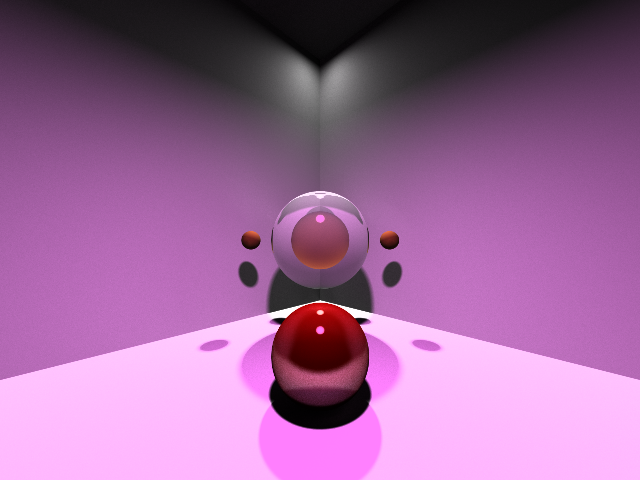
\includegraphics[width=8cm]{figures/pink_norm}}
  \caption{Varying light source colors}
  \label{fig:lightcolor}
\end{figure}

Figure \ref{fig:lightcolor} clearly shows what happens when the light
source color is varied. The most apparent results can be seen in the
shadows cast by the objects. Shadows caused by the white light source,
but visible to the pink light source will have a pink tint.

\section{Rendering speed}

This table will show rendering times for different settings running
single-threaded to have a fair comparison even though other processes
might be running on the computer.

% Tabell med lite olika inställningar och tider

Table REF clearly shows the effect on rendering time of increasing the number of viewing rays.

\section{Normalization}

The estimators in the direct and indirect illumination algorithm
should be normalized with the PDF of the Monte Carlo scheme. This is
ignored though for indirect illumination since it produces some
strange results but a difference can clearly be seen between an image
without normalized direct illumination and one without.

\begin{figure}
  \centering
  \subfloat[With normalization]{\label{fig:norm}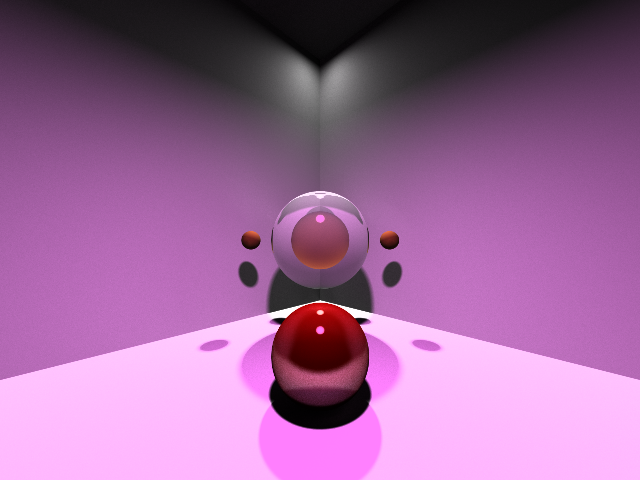
\includegraphics[width=8cm]{figures/pink_norm}}                
  \subfloat[Without normalization]{\label{fig:nnorm}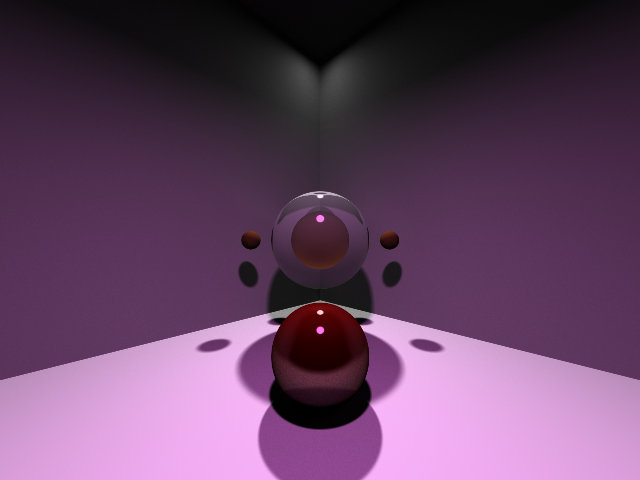
\includegraphics[width=8cm]{figures/pink_nnorm}}
  \caption{Normalized vs. Not normalized}
  \label{fig:normcomp}
\end{figure}

In figure \ref{fig:normcomp} it can be seen that the normalization
(figure \ref{fig:norm}) gives much more accurate color
reproduction. This is natural since the normalization in this case,
with uniform selection of light sources and uniform sampling of
point on light source, is a multiplication by a constant number.

\chapter{Discussion}
\label{ch:discussion}

Rendering an image with a raytracing algorithm can be a quite tedious
process and we have become aware of that as can be seen in table
REFERENCE. Since ray tracing is a view-dependent algorithm, every
pixel is totally independent of other pixels. To improve speed,
threading should be implemented and it
is one of the first improvements that this ray tracer will undergo. It
has already been prepared for by dividing the image into tiles which
makes it possible to independently calculate each tile.

As can be seen in the above image, there is no caustic effects. To
improve realism, a photon mapper could be added to the ray
tracer. This is the improvement that will probably have the biggest
impact on the visual result.

Polygonal object is an improvement to the software to be able to
produce more visually interesting results. This is not much work to do
since the intersection between ray and triangles are already included.

To better be able to control the scene, implementation of an xml
format called flaxxml has been started. It is not finished so it is
not included now but will probably be included in the near future.

Speed in intersection tests are another important aspect in ray
tracing. Our idea is to implement a BSP-tree for partitioning space
and an octree to subdivide meshes. This can be a drastic improvement
to rendering speed especially with polygonal objects containing many
polygons. The BSP-tree is useful for not having to test intersection
with every object in the scene but only those objects in the same
subspace as the launched ray.

To reduce the noise in images that can at times be extensive, BRDF
sampling of the hemisphere could be used. This would more accurately
sample the actual material and lower the variance and thus the noise.

The same holds for improving the soft shadows produced by the direct
illumination stage of the algorithm. Another sampling scheme could
have been used to lower the variance and thus the noise.

Talking of noise, a better random number generator should be
used. Experiments with a Mersenne-Twister RNG have been carried out
and the Mersenne-Twister RNG is actually implemented. However it did
not produce the wanted results, probably due to incorrect usage, so it
was not used. More experiments should be carried out with the
Mersenne-Twister RNG to try to incorporate it and use it in a correct way.

Better BRDFs can also be used. As said, an attempt on implementing a
Cook-Torrance shader was made. After reading the original paper by
Cook and Torrance, some new light has been shed on the problem (pardon
the bad humor). An attempt on implementing this could be made.

On the transparent side of the BRDF, we use only a constant and if the
Cook-Torrance shader is implemented, that can instead be used for more
correctly representing the light transport in transparent objects.

We feel very satisfied though with the results produced, since the
time frame was limited and the above items will probably be
implemented in the future. During the implementation we have learned a
lot and it has been both stimulating and sometimes frustrating to work
with. We have learned the hard way that it is hard (but very possible)
to debug a ray tracer.

Some good things that we are satisfied with in this project is among
other things, choosing SDL for interactive rendering. If we had not
done that, the debugging would have taken a lot more time since we
would have to wait for each render before getting results.

We also feel that the ray tracer is extendable since the class design
of it is well thought through.

% References
\bibliographystyle{ieeetr}
\bibliography{refs}

\end{document}

Maybe we should cite total compendium?